\hypertarget{sec:lrfk-methods}{%
\section{Methods}\label{sec:lrfk-methods}}

To evaluate thermodynamic averages I perform classical Markov Chain Monte Carlo random walks over the space of spin configurations of the LRFK model, at each step diagonalising the effective electronic Hamiltonian~\autocite{maskaThermodynamicsTwodimensionalFalicovKimball2006}. Using a Binder-cumulant method~\autocite{binderFiniteSizeScaling1981,musialMonteCarloSimulations2002}, I demonstrate the model has a finite temperature phase transition when the interaction is sufficiently long ranged. In this section I will discuss the thermodynamics of the model and how they are amenable to an exact Markov Chain Monte Carlo method.

\hypertarget{thermodynamics-of-the-lrfk-model}{%
\subsection{Thermodynamics of the LRFK Model}\label{thermodynamics-of-the-lrfk-model}}

\hypertarget{fig:raw_steps_single_flip}{%
\begin{figure}
\centering
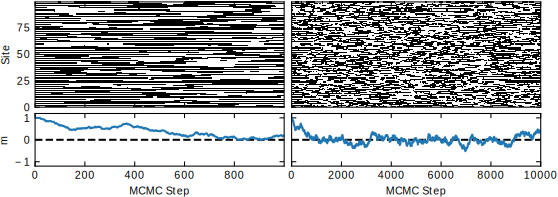
\includegraphics[width=1\textwidth,height=\textheight]{figure_code/fk_chapter/lsr/pdf_figs/raw_steps_single_flip}
\caption[{Comparison of different proposal distributions}]{Two MCMC walks starting from the CDW state for a system with \(N = 100\) sites and 10,000 MCMC steps but at a temperature close to but above the ordered state (left column) and much higher than it (right column). In this simulation only a single spin can be flipped per step according to the Metropolis-Hastings Algorithm. The staggered magnetisation \(m = N^{-1} \sum_i (-1)^i \; S_i\) order parameter is plotted below. At both temperatures the thermal average of m is zero, while the initial state has m = 1. The higher temperature allows the MCMC to converge more quickly and to fluctuate about the mean with a shorter autocorrelation time. \(t = 1, \alpha = 1.25, T = {2.5,5}, J = U = 5\)}
\label{fig:raw_steps_single_flip}
\end{figure}
}

The classical Markov Chain Monte Carlo (MCMC) method which we discuss in the following allows us to solve our long-range FK model efficiently, yielding unbiased estimates of thermal expectation values.

Since the spin configurations are classical, the LRFK Hamiltonian can be split into a classical spin part \(H_s\) and an operator valued part \(H_c\).

\[\begin{aligned}
H_s& = - \frac{U}{2}S_i + \sum_{i, j}^{N} J_{ij} S_i S_j \\
H_c& = \sum_i U S_i c^\dagger_{i}c_{i} -t(c^\dagger_{i}c_{i+1} + c^\dagger_{i+1}c_{i}) \end{aligned}\]

The partition function can then be written as a sum over spin configurations, \(\vec{S} = (S_0, S_1...S_{N-1})\):

\[\begin{aligned}
\mathcal{Z} = \mathrm{Tr} e^{-\beta H}= \sum_{\vec{S}} e^{-\beta H_s} \mathrm{Tr}_c e^{-\beta H_c} .\end{aligned}\]

The contribution of \(H_c\) to the grand canonical partition function can be obtained by performing the sum over eigenstate occupation numbers giving \(-\beta F_c[\vec{S}] = \sum_k \ln{(1 + e^{- \beta \epsilon_k})}\) where \({\epsilon_k[\vec{S}]}\) are the eigenvalues of the matrix representation of \(H_c\) determined through exact diagonalisation. This gives a partition function containing a classical energy which corresponds to the long-range interaction of the spins, and a free energy which corresponds to the quantum subsystem.

\[\begin{aligned}
\mathcal{Z} = \sum_{\vec{S}} e^{-\beta H_S[\vec{S}] - \beta F_c[\vec{S}]} = \sum_{\vec{S}} e^{-\beta E[\vec{S}]}\end{aligned}\]

\hypertarget{markov-chain-monte-carlo-and-emergent-disorder}{%
\subsection{Markov Chain Monte Carlo and Emergent Disorder}\label{markov-chain-monte-carlo-and-emergent-disorder}}

Classical MCMC defines a weighted random walk over the spin states \((\vec{S}_0, \vec{S}_1, \vec{S}_2, ...)\), such that the likelihood of visiting a particular state converges to its Boltzmann probability \(p(\vec{S}) = \mathcal{Z}^{-1} e^{-\beta E}\). Hence, any observable can be estimated as a mean over the states visited by the walk~\autocite{binderGuidePracticalWork1988,kerteszAdvancesComputerSimulation1998,wolffMonteCarloErrors2004},

\[\begin{aligned}
\label{eq:thermal_expectation}
\langle O \rangle & = \sum_{\vec{S}} p(\vec{S}) \langle O \rangle\\
                  & = \sum_{i = 0}^{M} \langle O\rangle \pm \mathcal{O}(M^{-\tfrac{1}{2}})
\end{aligned}\]

where the former sum runs over the entire state space while the later runs over all the state visited by a particular MCMC run.

\[\begin{aligned}
\langle O \rangle_{\vec{S}}& = \sum_{\nu} n_F(\epsilon_{\nu}) \langle O \rangle{\nu}
\end{aligned}\]

Where \(\nu\) runs over the eigenstates of \(H_c\) for a particular spin configuration and \(n_F(\epsilon) = \left(e^{-\beta\epsilon} + 1\right)^{-1}\) is the Fermi function.

The choice of the transition function for MCMC is under-determined as one only needs to satisfy a set of balance conditions for which there are many solutions~\autocite{kellyReversibilityStochasticNetworks1981}. Here, we incorporate a modification to the standard Metropolis-Hastings algorithm~\autocite{hastingsMonteCarloSampling1970} gleaned from Krauth~\autocite{krauthIntroductionMonteCarlo1998}.

The standard algorithm decomposes the transition probability into \(\mathcal{T}(a \to b) = p(a \to b)\mathcal{A}(a \to b)\). Here, \(p\) is the proposal distribution that we can directly sample from while \(\mathcal{A}\) is the acceptance probability. The standard Metropolis-Hastings choice is

\[\mathcal{A}(a \to b) = \min\left(1, \frac{p(b\to a)}{p(a\to b)} e^{-\beta \Delta E}\right)\;,\]

with \(\Delta E = E_b - E_a\). The walk then proceeds by sampling a state \(b\) from \(p\) and moving to \(b\) with probability \(\mathcal{A}(a \to b)\). The latter operation is typically implemented by performing a transition if a uniform random sample from the unit interval is less than \(\mathcal{A}(a \to b)\) and otherwise repeating the current state as the next step in the random walk. The proposal distribution is often symmetric so does not appear in \(\mathcal{A}\). Here, we flip a small number of sites in \(b\) at random to generate proposals, which is a symmetric proposal.

In our computations~\autocite{hodsonMCMCFKModel2021} the modification to this algorithm that we employ is based on the observation that the free energy of the FK system is composed of a classical part which is much quicker to compute than the quantum part. Hence, we can obtain a computational speed up by first considering the value of the classical energy difference \(\Delta H_s\) and rejecting the transition if the former is too high. We only compute the quantum energy difference \(\Delta F_c\) if the transition is accepted. We then perform a second rejection sampling step based upon it. This corresponds to two nested comparisons with the majority of the work only occurring if the first test passes. This modified scheme has the acceptance function \[\mathcal{A}(a \to b) = \min\left(1, e^{-\beta \Delta H_s}\right)\min\left(1, e^{-\beta \Delta F_c}\right)\;.\]

For the model parameters used, we find that with our new scheme the matrix diagonalisation is skipped around 30\% of the time at \(T = 2.5\) and up to 80\% at \(T = 1.5\). We observe that for \(N = 50\), the matrix diagonalisation, if it occurs, occupies around 60\% of the total computation time for a single step. This rises to 90\% at N = 300 and further increases for larger N. We therefore get the greatest speedup for large system sizes at low temperature where many prospective transitions are rejected at the classical stage and the matrix computation takes up the greatest fraction of the total computation time. The upshot is that we find a speedup of up to a factor of 10 at the cost of very little extra algorithmic complexity.

Our two-step method should be distinguished from the more common method for speeding up MCMC which is to add asymmetry to the proposal distribution to make it as similar as possible to \(\min\left(1, e^{-\beta \Delta E}\right)\). This reduces the number of rejected states, which brings the algorithm closer in efficiency to a direct sampling method. However it comes at the expense of requiring a way to directly sample from this complex distribution, a problem which MCMC was employed to solve in the first place. For example, recent work trains restricted Boltzmann machines (RBMs) to generate samples for the proposal distribution of the FK model~\autocite{huangAcceleratedMonteCarlo2017}. The RBMs are chosen as a parametrisation of the proposal distribution that can be efficiently sampled from while offering sufficient flexibility that they can be adjusted to match the target distribution. Our proposed method is considerably simpler and does not require training while still reaping some of the benefits of reduced computation.

\hypertarget{scaling}{%
\subsection{Scaling}\label{scaling}}

\hypertarget{fig:binder_cumulants}{%
\begin{figure}
\centering
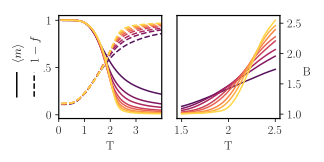
\includegraphics[width=1\textwidth,height=\textheight]{figure_code/fk_chapter/binder_cumulants/binder_cumulants}
\caption[{Binder Cumulants}]{(Left) The order parameters, \(\langle m^2 \rangle\)(solid) and \(1 - f\) (dashed) describing the onset of the charge density wave phase of the long-range 1D Falicov model at low temperature with staggered magnetisation \(m = N^{-1} \sum_i (-1)^i S_i\) and fermionic order parameter \(f = 2 N^{-1}|\sum_i (-1)^i \; \langle c^\dagger_{i}c_{i}| \rangle\) . (Right) The crossing of the Binder cumulant, \(B = \langle m^4 \rangle / \langle m^2 \rangle^2\), with system size provides a diagnostic that the phase transition is not a finite size effect, it's used to estimate the critical lines shown in the phase diagram \cref{fig:phase-diagram-lrfk}. All plots use system sizes \(N = [10,20,30,50,70,110,160,250]\) and lines are coloured from \(N = 10\) in dark blue to \(N = 250\) in yellow. The parameter values \(U = 5,\;J = 5,\;\alpha = 1.25\) except where explicitly mentioned.}
\label{fig:binder_cumulants}
\end{figure}
}

To improve the scaling of finite size effects, we make the replacement \(|i - j|^{-\alpha} \rightarrow |f(i - j)|^{-\alpha}\), in both \(J_{ij}\) and \(\kappa\), where \(f(x) = \frac{N}{\pi}\sin \frac{\pi x}{N}\). \(f\) is smooth across the circular boundary and its effect effect diminished for larger systems~\autocite{fukuiOrderNClusterMonte2009}. We only consider even system sizes given that odd system sizes are not commensurate with a CDW state.

To identify critical points we use the the Binder cumulant \(U_B\) defined by

\[
U_B = 1 - \frac{\langle\mu_4\rangle}{3\langle\mu_2\rangle^2}
\]

where \(\mu_n = \langle(m - \langle m\rangle)^n\rangle\) are the central moments of the order parameter \(m = \sum_i (-1)^i (2n_i - 1) / N\). The Binder cumulant evaluated against temperature is a diagnostic for the existence of a phase transition. If multiple such curves are plotted for different system sizes, a crossing indicates the location of a critical point while the lines do not cross for systems that don't have a phase transition in the thermodynamic limit~\autocite{binderFiniteSizeScaling1981,musialMonteCarloSimulations2002}.
